\chapter{Regulator klasyczny - PID}
\label{cha:regulator}

\section{Regulator PID}
Do pozycjonowania manipulatora zaproponowany został regulator składający się z dwóch równolegle połączonych regulatorów PID. Kiedy trzymana jest pełna szklanka, to na wyjście przekazywane jest sterowanie z pierwszego regulatora, a kiedy jest pusta to z drugiego. Regulatorom zadano inne nastawy po to, by w przypadku trzymania pełnej szklanki, ograniczyć przyspieszenie kątowe ramienia. Ma to na celu spełnienie warunku, by przyspieszenie było małe, aby nie wylać wody. Struktura obu regulatorów jest identyczna, wyrażona następujący wzorem:
\begin{equation}\label{key}
U(s) = (P + I \frac{1}{s} + D\frac{sN}{s+N}) \cdot E(s)
\end{equation}
gdzie:\newline
$U$ - transformata Laplace'a sterowania,\\
$E$ - transformata Laplace'a uchybu regulacji,\\
$P, I, D$ - współczynniki części proporcjonalnej, całkującej i różniczkującej.\\
\newline
Na podstawie przeprowadzonych symulacji przyjęto następujące nastawy regulatorów:\\
Regulator odpowiedzialny za pozycjonowanie ramienia z napełnioną szklanką:\\
$
P_1 = 3\\
I_1 = 0.2\\\
D_1 = 1.5\\
$\\
Regulator pozycjonujący ramie z pustą szklanką:\\
$
P_2 = 3\\
I_2 = 0.002\\
D_2 = 1\\
$

Pozycja zadana podawana na regulator manipulatora miała postać funkcji prostokątnej. Stwierdzono jednak, iż z uwagi na ograniczenie przyspieszenia, czas na ustalenie pozycji zadanej dla ruchu z pełną szklanką powinien być dłuższy. Na tej podstawie ustawiono czas pozycjonowania ramienia z napełnioną szklanką na 3~s, a czas powrotu ramienia na pozycję początkową na 2~s.\\
Na rysunku \ref{pid_res} przedstawiono odpowied\'z układu dla opisanych powyżej regulatorów.
Dla tak przyjętych nastaw regulatorów otrzymano następujące wartości wska\'zników jakości:\\
\newline
$J_1 = 3.847 \ [rad^2 \cdot s]$\\
$J_2 = 0.7587 [V^2 \cdot s]$\\
$J_3 = 4.606$\\
\begin{figure}[h]
	\centering
	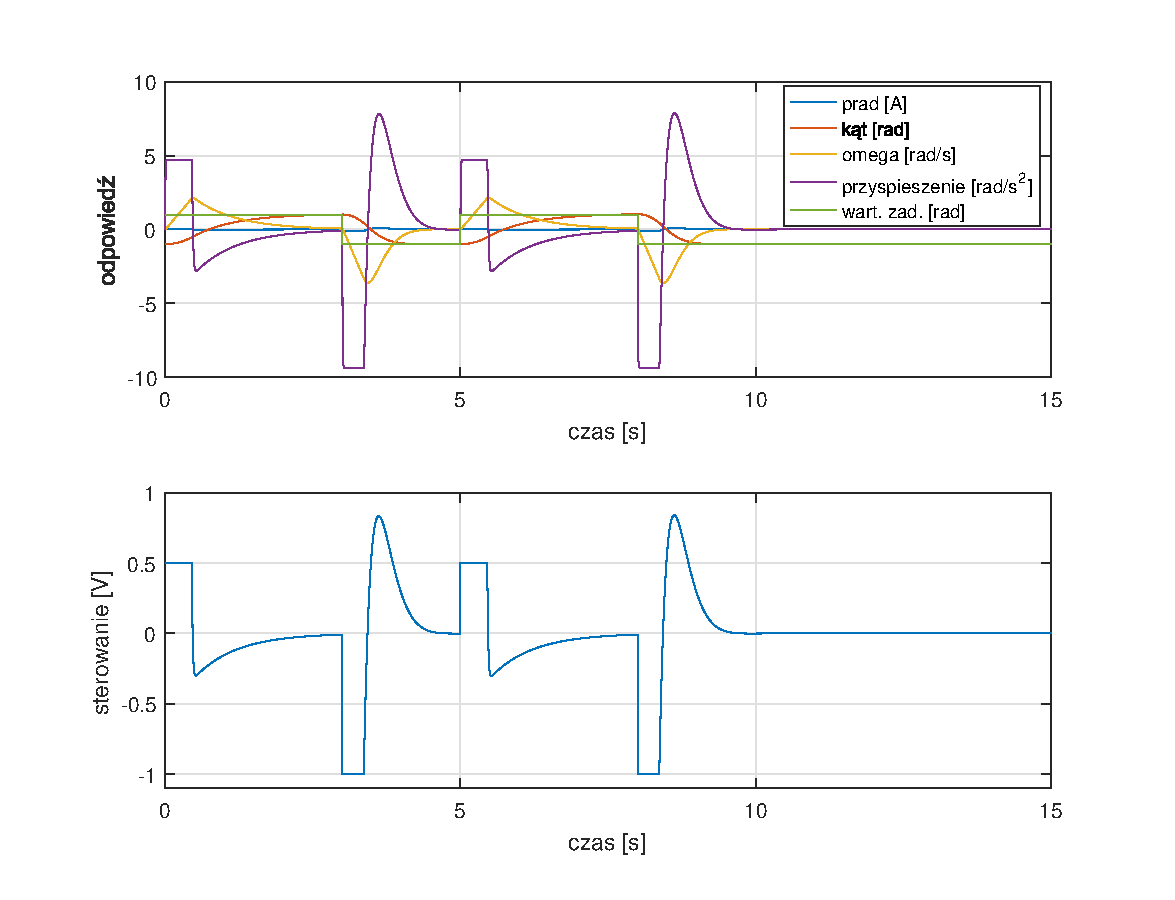
\includegraphics[scale = 0.9]{fig/pid_response.eps}
	\caption		
	{Wartości zmiennych stanu i sterowania.}
	\label{pid_res}
\end{figure} 